% !TeX spellcheck = nl_NL
 \chapter{Quadcopter platform}

%figuur aanvang thesis

Deze thesis is het vervolg op de thesis van W. De Gucht \cite{thesis:wouter}. In dit hoofdstuk wordt de situatie geschetst zoals die was bij de aanvang van deze thesis. Eerst wordt wat terminologie aangehaald, dan wordt de hardware van het platform overlopen en vervolgens wordt de functie van de belangrijkste softwareblokken belicht.

\section{Terminologie}

\begin{figure}[h]
	\centering
	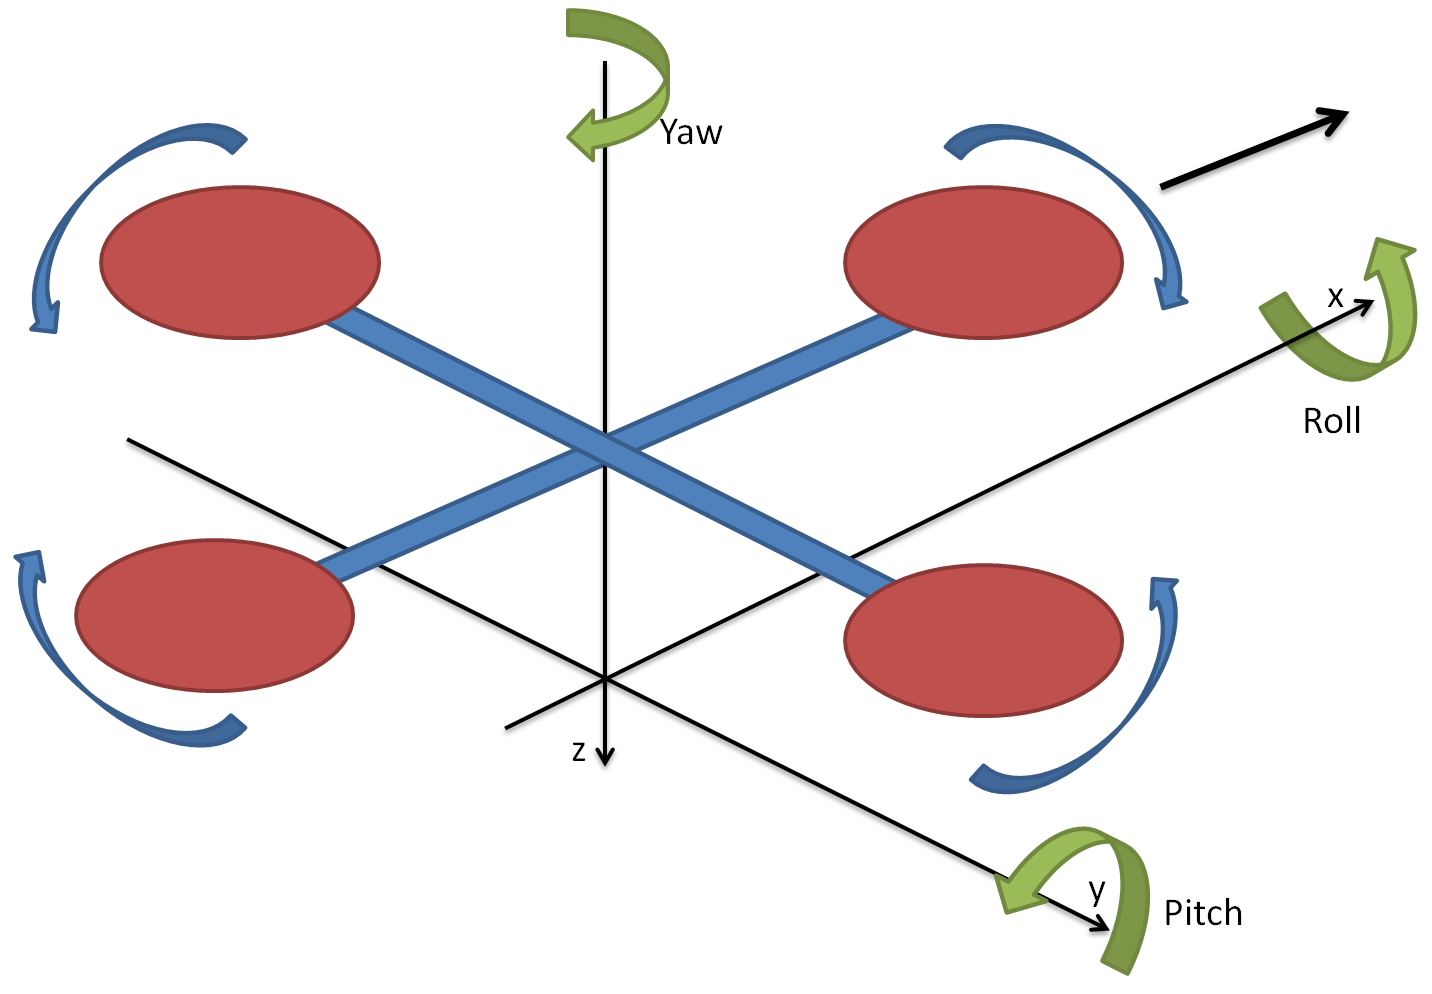
\includegraphics[width=0.6\linewidth]{yaw_pitch_roll}
	\caption{Schematische voorstelling van een quadcopter waarop het gebruikte assenstelsel en roll, pitch en yaw zijn aangeduid.}\label{fig:yaw_pitch_roll}
\end{figure}
\noindent Er wordt een rechtshandig assenstelsel gehanteerd, te zien op figuur \ref{fig:yaw_pitch_roll}, waarbij de z-as naar de grond is gericht. Binnen de aerodynamica wordt gebruik gemaakt van de hoeken \textit{roll}, \textit{pitch} en \textit{yaw} om de positie ten opzichte van de grond van een vliegend toestel uit te drukken. De namen van die hoeken worden ook in deze thesis gehanteerd. De roll is de rotatie rond de x-as, de pitch rond de y-as en de yaw rond de z-as. De snelheid waarmee een motor draait, krijgt de naam \textit{throttle}. Yaw, pitch, roll en de throttle van de vier motoren vormen samen het \textit{gedrag} van de quadcopter.

\section{Hardware}
In deze sectie komt de hardware van het platform aan bod. Er wordt een onderverdeling gemaakt op basis van de functie van de componenten. Het eerste deel, de quadcopterbasis, bestaat uit het frame, de motoren, de \textit{Electronic Speed Controllers} (ESC's) en de batterij. Het tweede deel, de quadcoptersturing omvat de hardware componenten die instaan voor het regelen van het vlieggedrag van het platform: de \textit{Raspberry Pi} (RPi) en de \textit{Ardupilot Mega} (APM). Alle componenten (behalve het frame) worden weergegeven op figuur \ref{fig:hardware}.

\begin{figure}[h]
	\centering
	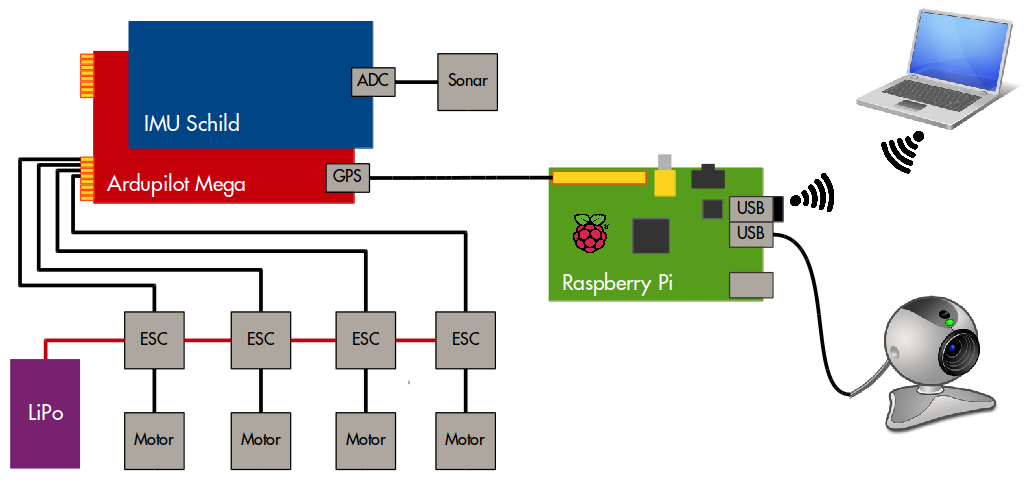
\includegraphics[width=0.9\linewidth]{hardware_whole}
	\caption{De hardware van het platform, schematisch voorgesteld.}
	\label{fig:hardware}
\end{figure}

\subsection{Quadcopterbasis}
Een overzicht van de quadcopterbasis wordt afgebeeld in figuur \ref{fig:quadbasis}. Alle onderdelen behalve de batterij worden weergegeven. Meestal wordt de batterij ergens onderaan of bovenaan het platform bevestigd net voor het vliegen.

\begin{figure}[ht]
	\centering
	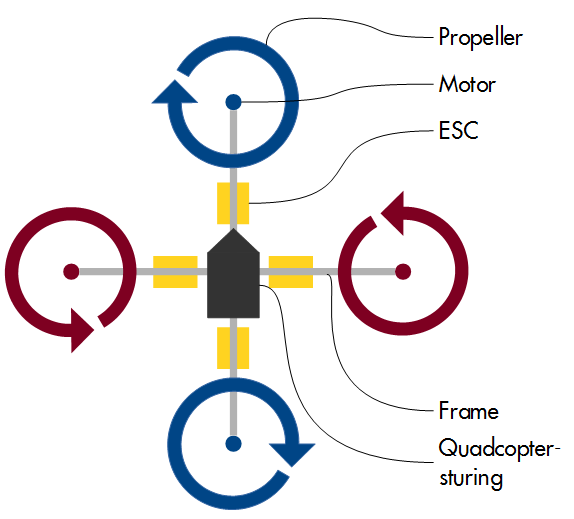
\includegraphics[width=0.50\linewidth]{quad}
	\caption{Overzicht van de quadcopterbasis.}
	\label{fig:quadbasis}
\end{figure}


\subsubsection{Frame}
De basis van de quadcopter is een \textit{plus-vormig} frame zoals te zien is in figuur \ref{fig:quadbasis}. In het midden van het frame is een ruimte voorzien voor het bevestigen van de elektronica die nodig is voor de sturing van het platform. Zoals het hoort staat op iedere arm een motor.

\subsubsection{Motoren}
Er wordt gebruik gemaakt van brushless DC motoren. Deze motoren maken geen fysisch contact om de ompoling in de kern te cre\"eren. Hierdoor is dit type motor erg efficient. De motoren vragen een maximale stroom van \SI{10}{A}.

\npar Aan iedere motor is een propeller bevestigd. Twee ervan moeten draaien in wijzerzin, de andere twee in tegenwijzerzin. De draairichting van de propellers is aangeduid op figuur \ref{fig:quadbasis}. Moesten alle vier de rotoren in dezelfde richting draaien, dan zou de quadcopter voortdurend rond zijn as roteren. De propellers die draaien in wijzerzin compenseren dus de draaiimpuls van die in tegenwijzerzin (omgekeerd geldt hetzelfde).

\subsubsection{ESC's}
Op alle vier de armen is een \textit{Electronic Speed Controller} (ESC) bevestigd. Het zijn \SI{20}{A} ESC's. Ze kunnen dus zeker genoeg stroom leveren om de motoren op hun snelst te laten werken.

\npar De ESC's moeten een \textit{Pulse Width Modulated} (PWM) signaal omzetten in een driefasig stroomsignaal. Dit laatste signaal zorgt ervoor dat de spoelen van de motoren afwisselend stroom krijgen en de motoren dus aan het draaien gaan. De duty cycle van het PWM signaal bepaalt de frequentie van het driefasig signaal dat een motor ontvangt. Hoe hoger de duty cycle, hoe hoger de frequentie van het driefasig signaal en hoe sneller de motor zal draaien.

\subsubsection{Batterij}
Om het platform te voeden wordt een 1000\,mAh lithium-ion-polymeer (LiPo) batterij gebruikt. Deze soort batterij kan indien nodig de \SI{40}{A} leveren die de motoren nodig hebben als ze op hun snelst werken.

\subsection{Quadcoptersturing} \label{sec:quadcoptersturing}
De sturing van het platform is onder te verdelen in twee delen. Op de eerste plaats is er de \textit{Ardupilot Mega} (APM) met bijhorend \textit{Inertial Measurements Unit} (IMU) schild. Deze twee bordjes staan in voor de controle van het vlieggedrag van de quadcopter. Op de tweede plaats is er de \textit{Raspberry Pi} (RPi). Deze \textit{single board computer} (SBC) wordt gebruikt om het gewenste vlieggedrag door te geven aan de APM. Bovendien wordt de RPi ook gebruikt om de snelheid van het platform te berekenen. Die berekende snelheid wordt door de APM gebruikt om de quadcopter in de ruimte te lokaliseren en eventuele drift ten opzichte van de gewenste positie te compenseren.

\subsubsection{Quadcopter sturen}
Een quadcopter kan op eenvoudige manier gestuurd worden. Om naar links, rechts, voor en achter te vliegen, kan gewoon de snelheid van \'e\'en motor aangepast worden. Figuur \ref{fig:navigate} (links) geeft dit weer een voorwaartse beweging. Door de snelheid van de achterste motor op te drijven zal de pitch verkleinen. De quadcopter kantelt naar voor. De propellers stuwen lucht nu deels naar achter. Als reactie vliegt de quadcopter naar voor. Door rotoren met dezelfde draaizin even te versnellen kan de yaw veranderd worden. Dit omdat de torsie in die draaizin dan niet wordt opgehoffen door de motoren met de andere draaizin. Figuur \ref{fig:navigate} (rechts) geeft dit weer.

\begin{figure}
	\begin{center}
		\subfigure{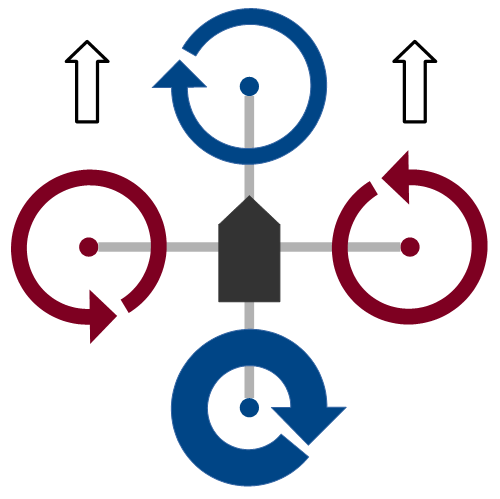
\includegraphics[width=0.40\linewidth]{navigate2}}
		\hspace*{0.1\linewidth}
		\subfigure{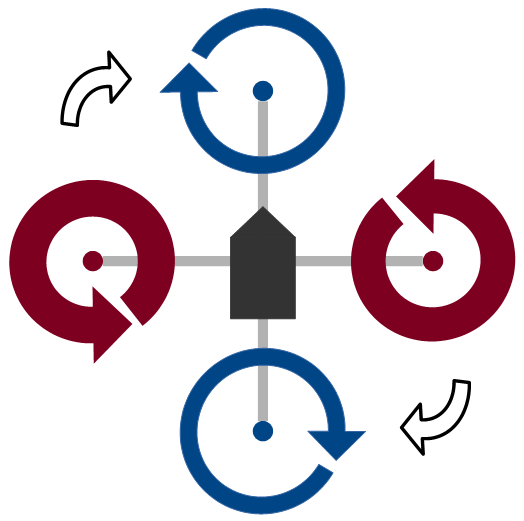
\includegraphics[width=0.40\linewidth]{navigate1}}
	\end{center}
	\centering
	\caption{Om een quadcopter vooruit te laten vliegen, moet de throttle van de achterste motor opgedreven worden (links). Om een quadcopter te laten roteren om de z-as moet de throttle van de rotoren in wijzerzin verschillen van die in tegenwijzerzin (rechts).}
	\label{fig:navigate}
\end{figure}

\subsubsection{Ardupilot Mega en IMU schild}
De APM, afgebeeld op figuur \ref{fig:APMIMU} (links), is het brein van de quadcopter. Het bordje heeft twee microcontrollers. De ATmega2560 is hiervan de belangrijkste. Het is een 8-bit microcontroller die alle inkomende data ontvangt en verwerkt. Hier wordt het gedrag bijgestuurd om het gewenste vlieggedrag te bekomen. De controlesignalen die bestemd zijn voor de motoren gaan naar de tweede microcontroller, de ATmega328. Deze controller moet ervoor zorgen dat deze signalen omgezet worden in PWM signalen. Dankzij deze tweede component, wordt de ATmega2560 minder belast en blijft er meer rekenkracht over voor berekeningen met betrekking tot stabilisatie.

\begin{figure}
	\centering
	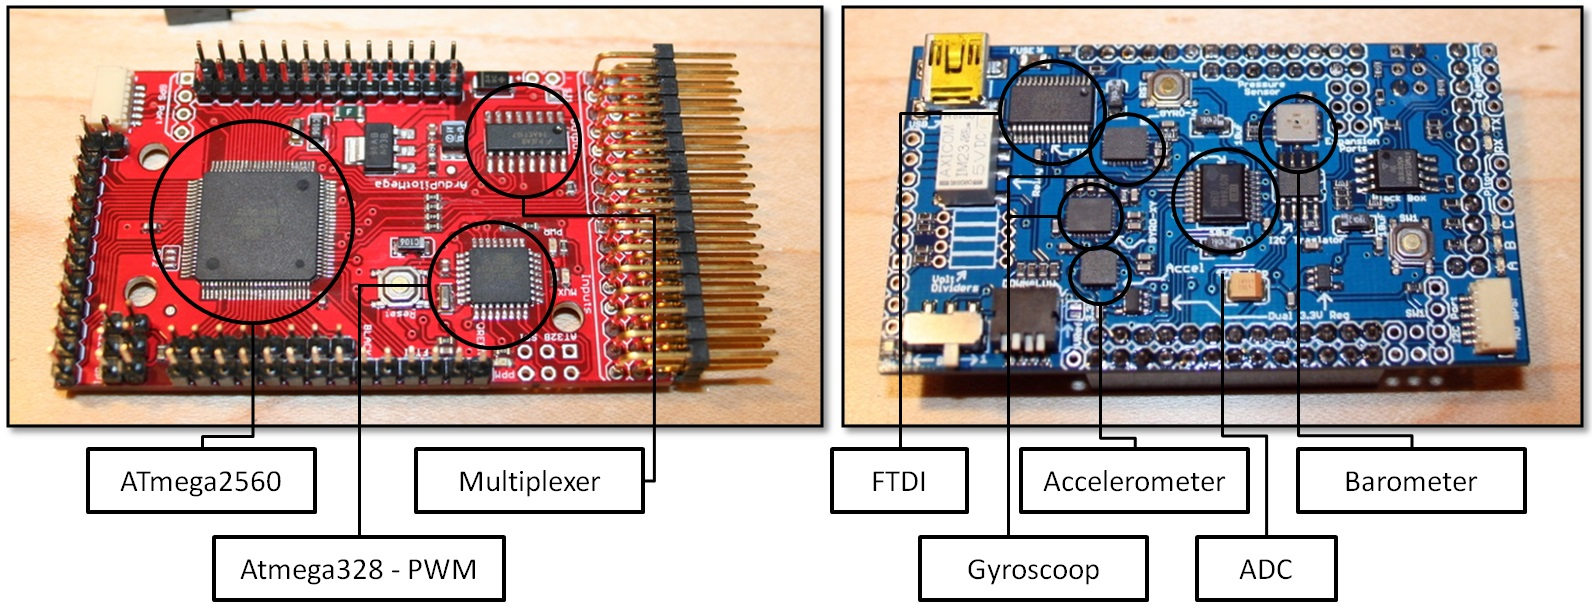
\includegraphics[width=0.8\linewidth]{APMIMU}
	\caption{De Ardupilot Mega(links) en het Inertial Measurements Unit schild(rechts) met hun belangrijkste componenten aangeduid op de figuur.}
	\label{fig:APMIMU}
\end{figure}

\npar De APM ontvangt data van de RPi via een seri\"ele verbinding. Deze verbinding is aangesloten op de APM waar normaal een GPS ontvanger moet komen. De APM kan ook sensoren uitlezen die op het IMU schild aanwezig zijn.

\npar Het IMU schild, ook weergegeven in figuur \ref{fig:APMIMU} (rechts),  beschikt over een gyrscoop waarmee de hoeksnelheid ten op zichte van alle assen kan gemeten worden. Er is ook een tri-axiale accelerometer die de versnelling in drie richtingen kan meten, in de richting van de x-as, y-as en de z-as. Bovendien wordt er ook een sonar verbonden die de hoogte van de quadcopter meet ten opzichte van de grond.

\subsubsection{Raspberry Pi}
De Raspberry Pi is \'e\'en van de bekendste SBC's op de markt. Omdat er een linux installatie op kan draaien is het eenvoudig om randapparatuur aan te sluiten. De RPi wordt voorzien van een camera die als input kan dienen voor optical flow. Voor communicatie met de APM is er zoals hierboven vermeld een seri\"ele verbinding voorzien. Er is ook een WiFi-dongle aanwezig om communicatie met de PC mogelijk te maken. De RPi met bijhorende randapperaten staat ook afgebeeld op figuur \ref{fig:hardware}.

\npar In de loop van de thesis werd de RPi\,2 uitgebracht. Deze SBC is veel krachtiger dan zijn oudere variant. Ter vergelijking worden de specificaties van de RPi\,1 en de RPi\,2 weergegeven in tabel \ref{table:RP1vsRPI2}. Naar het einde van deze thesis toe zal het gebruik van de nieuwe versie noodzakelijk worden.

\begin{table}[h]
	\caption{Vergelijking tussen aanvankelijk gebruikte RPi en het nieuwste model op de markt.} \label{table:RP1vsRPI2}
	\centering
	\begin{tabular}{lcc}
		\cr
		\hline
		& Raspberry Pi Model B & Raspberry Pi 2 Model B \\
		\hline
		CPU & 700 MHz & 900 MHz (Quadcore) \\
		RAM & 512 MB & 1 GB \\
		USB 2.0 poorten & 2 & 4 \\
		Stroomvoorziening & 5V & 5V \\
		\hline
	\end{tabular}
\end{table}

\section{Software}
In deze sectie worden alle aspecten van de quadcoptersturing uitgelegd. Hoe de quadcopter stabiel wordt gehouden en hoe er met het platform wordt gecommuniceerd. Zoals al eerder werd aangehaald, zijn de APM en de RPi de hardware componenten die instaan voor de sturing. Hun functie binnen het geheel komt hieronder ook in die volgorde aan bod.

\subsection{Ardupilot Mega} \label{sec:softAPM}
Binnen de APM kan er opgesplitst worden in twee delen. De software die instaat voor stabilisatie draait binnen de APM controlelus. Daarnaast is er ook nog de gebruikerlus. Hierin kan het gedrag van de quadcopter geprogrammeerd worden om uiteindelijk een autonoom platform te bekomen. De volledige architectuur van de APM wordt weergegeven in figuur \ref{fig:APMsoftware}.

\begin{figure}[h]
	\centering
	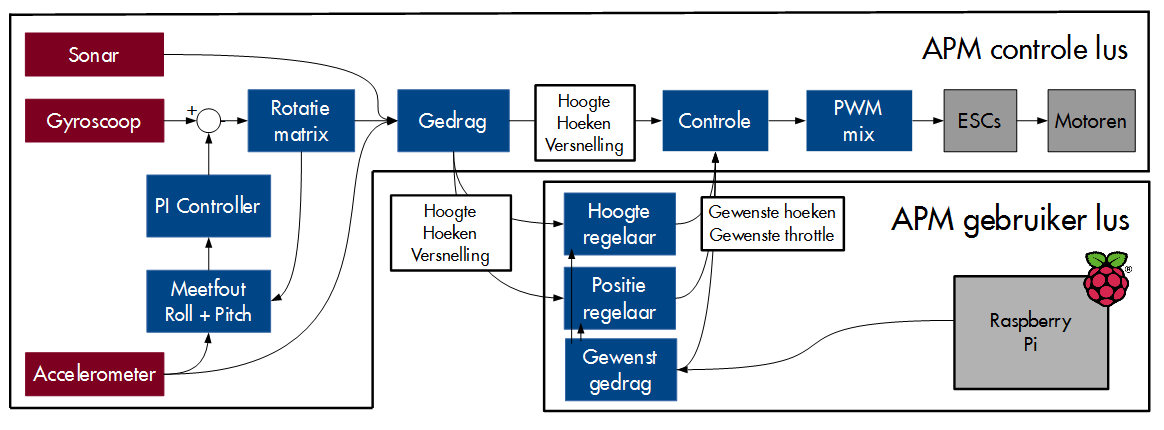
\includegraphics[width=\linewidth]{APMsoftware}
	\caption{Architectuur van de Ardupilot Mega.}
	\label{fig:APMsoftware}
\end{figure}

\subsubsection{Ardupilot controlelus}
In de rotatiematrix worden de hoeken ten opzichte van het referentiestelsel bijgehouden. Deze matrix wordt constant ge\"updatet met de hoeksnelheden gemeten door de gyroscoop. De rotatiematrix moet orthogonaal zijn. De meetfout van de gyroscoop moet dus gecompenseerd worden. Dit gebeurt door renormalisatie toe te passen. De fout op de hoeken wordt hier gecompenseerd door ervoor te zorgen dat de rotatiematrix opnieuw orthogonaal wordt.

\npar De rotatiematrix is nu reeds vrij betrouwbaar. Er zit wel nog een zekere drift op. Om deze drift te compenseren wordt accelerometerdata gebruikt. De zwaartekracht kan gemeten worden, deze is evenwijdig met de z-as van het referentiestelsel. Hieruit kan dan de meetfout op pitch en roll gehaald worden. De meetfout wordt dan met een PI-regelaar teruggevoerd naar de rotatiematrix.

\npar De hoogte van het platform gemeten door de sonar, de hoeken berekend door de rotatiematrix en de accelerometerdata gemeten door de accelerometers worden doorgegeven aan het gedrag. In het gedrag kan dus de huidige toestand van het platform terug gevonden worden. De huidige toestand wordt in de gebruikerlus gebruikt om hoogte en positie van het platform te regelen. Het gedrag wordt ook naar de controle gestuurd.

\npar In de controle wordt het gedrag gebruikt om de corrigerende acties te berekenen die nodig zijn om de quadcopter stabiel te houden. Daarnaast neemt de controle ook het gewenste gedrag in acht. De snelheid waarmee iedere motor moet draaien wordt berekend. Het resultaat wordt dan doorgegeven naar de PWM mixer en omgezet in PWM signalen. De ESC's maken van die PWM signalen de driefasige stroomsignalen waarmee de motoren bestuurd worden.

\subsubsection{Ardupilot gebruikerlus}
De gebruikerlus neemt als ingang het gedrag van de quadcopter. Zoals reeds werd vermeld bevat dit gedrag de hoogte, de hoeken ten opzichte van het referentiestelsel en de versnellingen in alle richtingen. Daarnaast wordt ook optical flow data ontvangen van de RPi.

\npar De hoogte PID-regelaar neemt de hoogte als input. De gewenste hoogte kan via de RPi worden ingesteld. De huidige hoogte wordt gecorrigeerd door de gewenste throttle aan te passen.

\npar Een positie PID-regelaar neemt de hoeken, de versnelling en de optical flow data afkomstig van de RPi als input. Met deze informatie kan de exacte locatie van de quadcopter berekend worden. Ook hier wordt de exacte positie vergeleken met de setpoint ingesteld via de RPi. De positie kan gecorrigeerd worden door roll en pitch bij aan te passen. Als het platform van zijn gewenste positie wegdrift, dan moet deze PID-regelaar die drift tegenwerken.

\npar Het effectief berekenen van de locatie van het platform verdient nog een klein woordje uitleg. De optical flow data die gebruikt wordt voor de berekening van de locatie van het platform, bevat de optische snelheden $(OF_x)_{ongecomp.}$ en $(OF_y)_{ongecomp.}$ van het platform, gemeten over twee camerabeelden. Om hieruit de effectieve snelheid af te leiden moeten nog een aantal berekeningen gebeuren. Om de correcte snelheid af te leiden moet rekening gehouden worden met de roll, de pitch en de hoogte van de quadcopter. Dit wordt verduidelijkt door figuur \ref{fig:invloed}.

\begin{figure}[h]
	\centering
	\subfigure[Invloed van roll en pitch op optical flow snelheid.]{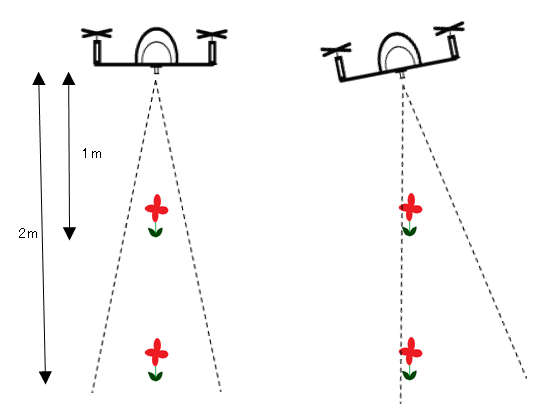
\includegraphics[width=0.48\linewidth]{invloedhoek}}
	\hspace{0.01\linewidth}
	\subfigure[Invloed van hoogte op optical flow snelheid.]{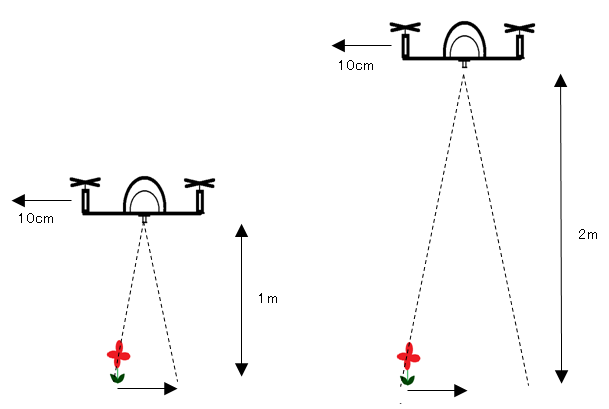
\includegraphics[width=0.48\linewidth]{invloedhoogte}}
	\caption{Bij het omzetten van optical flow data naar een effectieve snelheid moet rekening gehouden worden met roll en pitch(a) en met de hoogte(b) van het platform.} \label{fig:invloed}
\end{figure}

\npar Ten eerste moet het verschil in roll en pitch tussen de twee cameraopnames gecompenseerd worden. Als dit niet wordt gedaan, dan klopt de door optical flow gedetecteerde snelheid niet. Stel dat het platform een beetje kantelt, maar toch op dezelfde positie in de lucht blijft hangen. Er zal toch optical flow gedetecteerd worden, terwijl het platform zich eigenlijk niet verplaatst. Dit probleem wordt afgebeeld op figuur \ref{fig:invloed}(a). Formules \eqref{eq:comproll} en \eqref{eq:comppitch} kunnen gebruikt worden om de ontvangen optische snelheden te compenseren met $\omega_{roll}$ en $\omega_{pitch}$, de roll- en pitchhoeksnelheid \cite{thesis:wouter}. Nu geweten is hoe de optische snelheid gecompenseerd moeten worden, moet het goeie moment voor deze compensatie nog worden uitgekozen. Omdat de optical flow data van de RPi moet komen, zit er een zekere delay op. Deze delay blijkt twee tijdstappen groot te zijn. Hierbij is \'e\'en tijdstap de tijd tussen twee ontvangen optical flow vectoren.

\begin{equation}
OF_x = (OF_x)_{ongecomp.} - \omega_{pitch} \cdot \frac{R_x}{K_x}
\label{eq:comproll}
\end{equation}
\begin{equation}
OF_y = (OF_y)_{ongecomp.} - \omega_{roll} \cdot \frac{R_y}{K_y}
\label{eq:comppitch}
\end{equation}

\npar Vervolgens moet de snelheid die nu nog uitgedrukt is in pixels per seconde omgezet worden in meter per seconde. De hoogte $h$, de kijkhoeken $K_x$ en $K_y$ en de resolutie $R_x$x$R_y$ van de gebruikte camera zijn gekend. Na enkele simpele goniometrische berekeningen blijkt dat forumles \eqref{eq:vx} en \eqref{eq:vy} de snelheid in meter per seconde geven \cite{thesis:wouter}.

\begin{equation}
v_x = OF_x \cdot \frac{2 \cdot h \cdot \tan(K_x/2)}{R_x}
\label{eq:vx}
\end{equation}
\begin{equation}
v_y = OF_y \cdot \frac{2 \cdot h \cdot \tan(K_y/2)}{R_y}
\label{eq:vy}
\end{equation}

\subsection{Raspberry Pi} \label{sec:softRPi}

Figuur \ref{fig:RPIloop} geeft de architectuur van de RPi weer. Optical flow wordt berekend in \textit{OpticalFlow.cpp} en doorgestuurd naar het serieel model. $Keyboard.py$ kijkt naar input van de gebruiker en plaatst die in de wachtrij van het serieel model. Het serieel model, $SerialModel.py$, beheert het verkeer tussen de APM en de verschillende processen op de RPi.

\begin{figure}[h]
	\centering
	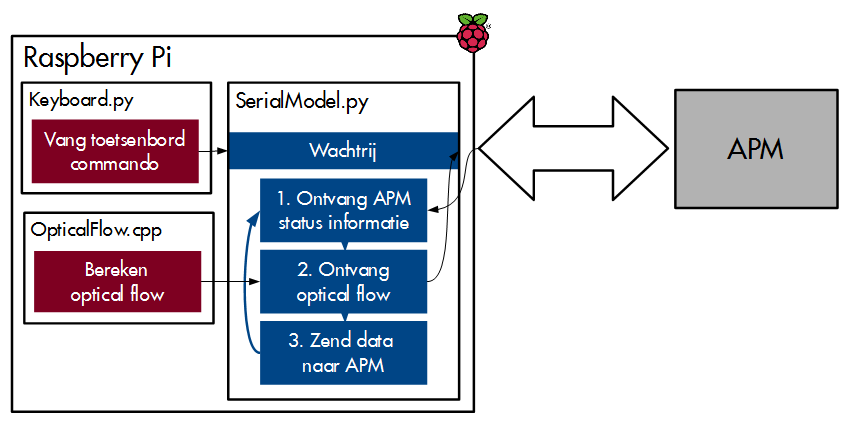
\includegraphics[width=0.8\linewidth]{RPIloop.png}
	\caption{Architectuur van de Raspberry Pi.}
	\label{fig:RPIloop}
\end{figure}

\npar De Raspberry Pi vervult hiermee vier taken, hieronder gerangschikt met dalende prioriteit:
\begin{itemize}
\item[1.] Optical flow berekenen
\item[2.] Optical flow data verzenden naar APM.
\item[3.] Uitprinten of opslaan van de statusinformatie afkomstig van APM.
\item[4.] Commando's van de computer verzenden naar APM.
\end{itemize}

\noindent Taak 1: het berekenen van optical flow, het algoritme voor deze berekening wordt uitgelegd in \ref{sec:OptFlow}. De APM verwacht de optische snelheid van het platform. De optische snelheid wordt telkens doorgestuurd naar de lus van het serieel model via een \textit{non-blocking send}. Op die manier kan het programma onmiddellijk aan de volgende berekening beginnen. In het serieel model wordt gebruik gemaakt van een \textit{blocking receive} bij het ontvangen van optical flow data. Op die manier wordt verzekerd dat de data doorgestuurd wordt naar de APM van zodra ze beschikbaar is.

\npar In de lus van het serieel model worden taken 2 tot 4 voortdurend uitgevoerd. Als er commando's worden ontvangen van de computer, worden die telkens achteraan in de wachtrij toegevoegd. Wanneer er optical flow data beschikbaar is, wordt die telkens vooraan in de wachtrij gezet en wordt de hele wachtrij verzonden. De mogelijke commando's en hun betekenis worden opgelijst in tabel \ref{table:oldcom}.

\begin{table}[h]
	\caption{Nieuwe commando's om het vlieggedrag te be\"invloeden.}\label{table:oldcom}
	\centering
	\begin{tabular}{cp{.3\linewidth}cp{.3\linewidth}}
		\cr
		\hline
		Commando & Betekenis & Commando & Betekenis \\
		\hline
		z & Verhoog pitch & s & Verlaag pitch\\
		q & Verhoog roll & d & Verlaag roll \\
		w & Verhoog yaw & x & Verlaag yaw \\
		a (auto) & Verhoog gewenste hoogte & e (auto) & Verlaag gewenste hoogte \\
		a (manueel) & Verhoog throttle & e (manueel) & Verlaag throttle\\
		c & Ga naar manuele modus & v & Ga naar manuele modus \\	
		r & Leg motoren aan & t & Schakel motoren uit \\	
		f & Print quadcopterstatus & & \\
		\hline				
	\end{tabular}
\end{table}

\npar Taak 3 spreekt voor zich, wanneer de APM statusinformatie ter beschikking stelt, wordt deze geprint en eventueel ook opgeslagen. Deze statusinformatie is heel handig voor het debuggen van de APM software. De statusinformatie kan ook gebruikt worden om het vlieggedrag na een vlucht visueel voor te stellen.

%sectie over de werking en implementatie van optical flow!!
\subsection{Optical flow} \label{sec:OptFlow}
Het belang van optical flow werd reeds aangewezen in \ref{sec:softAPM}. Het gebruikte algoritme voor het berekenen van optical flow snelheden wordt uit de doeken gedaan aan de hand van figuur \ref{fig:algOptFlow}.
%figuur met optical flow algoritme
\begin{figure}[h]
	\centering
	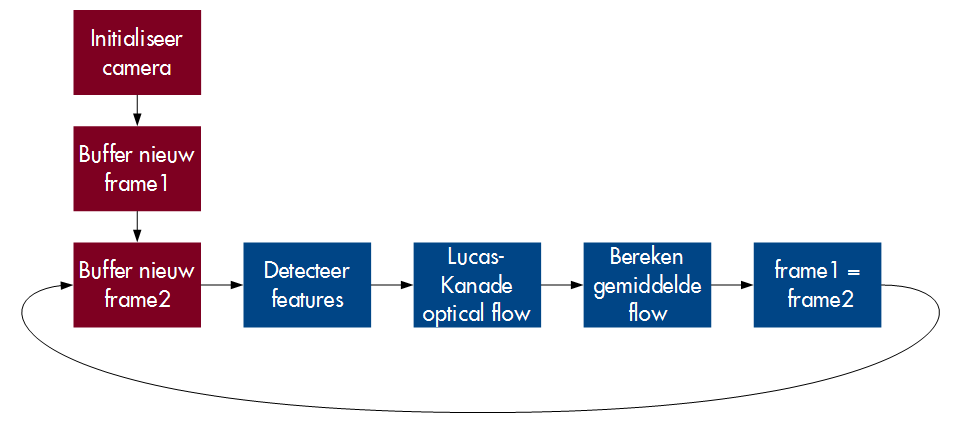
\includegraphics[width=0.8\linewidth]{algOpticalFlow}
	\caption{Het optical flow algoritme wordt in deze figuur grafisch voorgesteld.} \label{fig:algOptFlow}
\end{figure}

\npar Om te beginnen wordt de camera ge\"initialiseerd. Vervolgens worden de eerste twee frames in een buffer opgeslagen. Nu is alle nodige data beschikbaar om de eerste optical flow snelheidsvector te berekenen. 

\npar In het eerste frame wordt met de FAST detector \cite{paper:FAST} gezocht naar goede features. De werking van deze detector wordt in \ref{sec:FAST} kort uitgelegd. Eens features geselecteerd zijn, moeten die gezocht worden in het tweede frame. Wanneer de verplaatsing van iedere feature over de twee frames gekend is, wordt de gemiddelde optische verplaatsing berekend. Zoals reeds vermeld verwacht de PID-regelaar van de APM optische snelheden. De gemiddelde verplaatsing moet dus enkel nog gedeeld worden door de tijd tussen de twee frames. Eens de optical flow data is verstuurd kan er overgegaan worden naar het volgende frame. Het eerste frame wordt vervangen door het tweede, een nieuw frame wordt gebufferd en de hierboven beschreven stappen herhalen zich.

\npar Het zoeken van de optical flow tussen twee frames gebeurt zoals beschreven werd door J.Y. Bouguet in ``Pyramidal Implementation of the Affine Lucas Kanade Feature Tracker" \cite{paper:PyrLK}. Deze paper stelt een effici\"ente manier voor om de feature tracker voorgesteld door Lucas en Kanade \cite{paper:LK} te implementeren. De methode maakt gebruik van beeldpiramides. De geselecteerde features van het eerste frame worden eerst gezocht in een lage resolutie-kopie van het tweede frame. Wanneer een match gevonden wordt, moet enkel nog in de buurt deze match gezocht worden in de hogere resolutie-kopi\"en. Dit zorgt ervoor dat het zoeken van features in het tweede frame veel sneller gaat dan wanneer rechtstreeks in het oorspronkelijke frame gezocht zou worden.

\npar Zowel de FAST detector en de gebruikte optical flow implementatie zijn beschikbaar in de OpenCV bibliotheek \cite{url:opencv}. Het is dan ook niet meer dan logisch dat deze bibliotheek wordt gebruikt.

\section{Evaluatie van het platform}
Hoewel het platform bij het eind van de thesis van W. De Gucht, goed werkte, was dit helaas niet meer het geval bij aanvang van deze thesis. Er waren wat problemen om de APM werkende te krijgen. De code die reeds beschikbaar was op de APM, was geschreven voor het gebruik van de quadcopter met afstandsbediening. Een groot stuk moest herschreven worden omdat voor deze thesis geen afstandbediening wordt gebruikt. Bovendien werkte de communicatie tussen optical flow en het serieel model ook niet naar behoren. Dit stuk moest ook opnieuw worden geprogrammeerd.

%Beperkte rekenkracht RPi
\npar Uit het werk van W. De Gucht blijkt dat de RPi reeds 80\% van zijn totale rekenkracht nodig heeft voor het uitvoeren van het optical flow algoritme. Dit terwijl de resolutie van de gebruikte beelden slechts 160 bij 120 pixels bedraagt. Naast optical flow moet er ook nog gecommuniceerd worden met de APM. Omdat de processorkracht van de RPi gedeeld moet worden met een ander proces, is de uitvoeringssnelheid van het optical flow algoritme ver van optimaal. Er moet dus een manier bedacht worden om de RPi te ontlasten van het zware rekenwerk. Op die manier kan dan verzekerd worden dat het optical flow algoritme aan de optimale snelheid wordt uitgevoerd. De optimale snelheid is natuurlijk de maximale framerate van de gebruikte camera (\SI{30}{\Hz}).

%Tekorten voor uitbreiding naar omgevingsmapping --> misschien figuur toevoegen!!
\npar Het doel van deze thesis is om uiteindelijk aan omgevingsmapping te kunnen doen. Zoals reeds werd vermeld, moet het platform daarom op veilige manier autonoom in een ruimte kunnen rondvliegen. Momenteel worden gewenste positie en hoogte telkens ingesteld met behulp van een stapfunctie. Dit zorgt voor overshoot in het vlieggedrag, wat absoluut niet wenselijk is. Als de quadcopter iets te ver vliegt, kan hij bijvoorbeeld tegen een muur botsen. De positie- en hoogteregelaar moeten dus op een betere manier worden aangestuurd. Omgevingsmapping zou natuurlijk niet lukken zonder laserscanner of extra camera. Er moet dus nog een plaats voorzien worden op het platform waar de laserscanner gemonteerd kan worden.
